\documentclass[12pt,a4paper]{article}
\usepackage[margin=2.5cm]{geometry}
\usepackage{amsmath,amssymb,graphicx,setspace,palatino,float,subcaption, booktabs, titlesec,lineno}
\usepackage[colorlinks, allcolors = blue]{hyperref}
\usepackage{natbib}
\citestyle{egu}

\usepackage[usenames,dvipsnames]{xcolor}

\captionsetup[figure]{labelfont=bf,textfont={small,normalfont}}
%\captionsetup[subfigure]{labelsep=quad, labelfont={bf,small}, textfont=small, singlelinecheck=off, justification=raggedright, position=top}
%\renewcommand{\thesubfigure}{\Alph{subfigure}}

\renewcommand{\subsectionautorefname}{Section}
\renewcommand{\subsubsectionautorefname}{Section}
\titleformat{\paragraph}[hang]{\normalfont\normalsize\itshape}{\theparagraph}{0em}{}
\titlespacing*{\paragraph}{0pt}{1\baselineskip}{3pt}
\setlength{\parindent}{0pt}
\setlength{\parskip}{\baselineskip}


\newcommand{\cmnt}[1]{{\color{purple} #1}}

\renewenvironment{abstract}{%
  \normalsize
  \textbf{\large\abstractname\\[1em]} % with a normal space
}

\title{Neutral models of \textit{de novo} gene emergence suggest that gene evolution has a preferred trajectory}
\author{Bharat Ravi Iyengar$^1$, Erich Bornberg-Bauer$^{1,2}$}
\date{\small $^1$Institute for Evolution and Biodiversity, Westfalian Wilhelms -- University of M\"{u}nster, H\"{u}fferstrasse 1, 48149 M\"{u}nster, Germany\\ $^2$Max Planck-Institute for Biology T\"{u}bingen, T\"{u}bingen, Germany}

\begin{document}

\onehalfspacing

\setlength{\abovedisplayskip}{0pt}
\setlength{\belowdisplayskip}{1em}

\maketitle


\linenumbers

\section*{Abstract}
New protein coding genes can emerge from genomic regions that previously did not contain any genes, via a process called \textit{de novo} gene emergence. To synthesize a protein, DNA must be transcribed as well as translated. Both processes need certain DNA sequence features. Stable transcription requires promoters and a polydenylation signal, while translation requires at least an open reading frame (ORF). We develop mathematical models based on mutation probabilities, and the assumption of neutral evolution, to find out how quickly genes emerge and are lost. We also investigate the effect of the order by which DNA features evolve, and if sequence composition is biased by mutation rate. We rationalize how genes are lost much more rapidly than they emerge, and how genes with long ORFs preferentially arise in regions that are already transcribed. Our study not only answers some fundamental questions on the topic of \textit{de novo} emergence but also provides a modeling framework for future studies.



\section{Introduction}

Organisms evolve new traits by expanding their functional genome. Evolution of new genes is one of the ways by which new traits can emerge. The definition of a gene is complicated, and has been changing constantly \citep{genepostencode}. We use the following working definition of a gene: a gene is a region of the genome that gives rise to a functional product, that is an RNA or a protein. The next big challenge is to define what a function is, and how to classify gene functions. One of the easiest definition of a gene product's function is its ability to improve the survival of the organism under one or more environmental conditions \citep{deNovoFunction}. Proteins perform the most diverse kinds of molecular functions ranging from catalysis of biochemical reactions to formation of cellular structures \citep{berg}, whereas RNAs that do not encode proteins like mRNAs, or participate in protein synthesis like rRNAs and tRNAs, are mostly involved in regulation of gene expression \citep{fncel,Statello2021}.

In this study we focus on the evolution of genes that encode new proteins. New protein coding genes frequently arise via duplication of existing protein coding genes. These duplicated genes then genetically and functionally diverge from their parent genes by accumulating mutations \citep{Long2003,IAD}. Recently it has been shown that new protein coding genes can arise independent of gene duplication, from genomic sequences that did not previously encode any protein. This phenomenon is called \textit{de novo} gene emergence \citep{Tautz2011,Zhao2014,EBB-F1000,Vakirlis2017,vanOss}. \textit{De novo} protein coding genes can emerge from intergenic sequences, non-coding RNA genes, introns, and even regions that partially overlap with existing protein coding genes \citep{Tautz2011,Zhao2014,Vakirlis2017,vanOss,Prabh2019}. To express a protein, a genomic sequence should be transcribed as well as translated. Therefore, the gene needs sequence features that enable both these processes. 

\cmnt{The primary requirement for transcription is recruitment of RNA polymerase. This process is facilitated by DNA sequences called \citep{Promoters}. A part of the promoter, called the core promoter is the region that determines the start of transcription \citep{corepromoters}. Transcription can also be initiated without the requirement of a defined promoter sequence, and this process can occur throughout the genome \cite{PervasiveTranscription}. Even though pervasive transcription is widespread in eukaryotic genomes, most RNAs are quickly eliminated by RNA degrading enzymes \citep{RNAturnover}. Most eukaryotic mRNAs and long non-coding RNAs, are polyadenylated at their 3' termini, which makes them resistant to degradation. Polyadenylation, which also marks the end of transcription \citep{polyAterm}, is facilitated by sequences known as polyadenylation signals \citep{polyA}. In prokaryotes, the end of transcription is determined by sequences known as terminators \citep{ProkTerm}. Termination at an appropriate site is another fundamental requirement for a productive transcription.}

The second major requirement for protein expression is translation of the transcribed mRNA. The most fundamental requirement for translation is the presence of an open reading frame (ORF). Usually, an mRNA needs additional features to initiate protein synthesis. These features include ribosome binding sites in prokaryotes \citep{RBS}, and Kozak consensus sequences in eukaryotes \citep{kozak,kozakDroso,kozakHuman}. 

Although gain of transcription and translation features guarantees \textit{de novo} birth of a protein coding gene, it does not ensure that the gene would persist in the genome for many generations. The newly born gene can lose the features as easily as it gained them unless it has been fixed in the genome, for example via evolutionary selection. Specifically, if the protein synthesized by the \textit{de novo} gene provides a fitness advantage to the host organism, it will undergo positive selection \citep{deNovoFunction}. Simultaneously, the protein should have low toxicity and cost of synthesis, to survive purifying selection. A common mechanism by which protein mediated toxicity occurs is by misfolding and aggregation of proteins \citep{misfold1,misfold2}.

In this study we develop probabilistic models of \textit{de novo} gene emergence \cmnt{in eukaryotes}. We focus on \textit{de novo} genes emerging from non-genic sequences, also known as ``proto-genes'' \citep{protogenes,vanOss}. We model \textit{de novo} gene emergence as a two step process. In the first step, a non-genic DNA sequence gains transcriptional features that allows it to express an untranslated (non-coding) RNA. In the second step this non-coding RNA gene acquires translational features that allows it to express a protein. Alternatively, translational features can emerge in the non-genic DNA before transcriptional features. Specifically, we calculate the probabilities by which polyadenylation signals and ORFs emerge, and are lost, based on the rates at which different kinds of DNA mutations naturally occur (mutation bias). With these probabilities we estimate whether transcriptional and translational features preferentially evolve in a specific order. Using a similar approach, we calculate how random mutations affect protein composition. In our models, we assume that the proteins expressed from these proto-genes provide no fitness advantage and are not toxic to the host organism. Thus our models are based on neutral evolution. Our models predict that there is indeed a preferred sequence of DNA feature evolution during \textit{de novo} emergence, even under the assumption of neutrality.

\section{Results}

In this work, we developed mathematical models to estimate the rates and probabilities of \textit{de novo} gene emergence, as well as gene loss. A proto-gene emerges from non-genic DNA, when the latter mutates to gain sequence features necessary for transcription and translation \citep{protogenes,vanOss}. Both transcription and translation are complex processes involving many biomolecular complexes that work in concert. Here, we focus on the minimal requirements for these processes to occur. \cmnt{Experimental data show that transcription in eukaryotes can be initiated genome wide, especially in regions proximal to enhancers, and more specifically, in regions depleted of nucleosomes \citep{enhancers}. Thus transcription of many proto-genes can be initiated at a basal transcription rate, and may not require specific core promoters. Although transcription may be initiated without a core promoter, a stable RNA product often requires a poly-A tail that also facilitates RNA export to cytoplasm \citep{polyAterm,polyAexp}. This assumption is supported by experimental data, where the majority of detectably expressed proto-genes have polyadenylated RNAs \citep{Neme2016,Witt2019,PacoEnhancers,albaYeastdenovo}. Thus, we define a poly-A signal as the primary requirement for transcription such that it should exist but only at the end of a transcribed region.} For translation, we only require the gene to have an open reading frame (ORF). We only focus on intronless genes in this study. 

Using simple probability models, we calculate the likelihood of finding the sequence features that facilitate \textit{de novo} gene emergence by random chance, and the rate at which these features are gained and lost due to random mutations. These probability models are essentially described by two kinds of probability. First is the probability of finding a DNA sequence feature (such as the poly-A signal or an ORF; \autoref{methprob}). This probability depends on the nucleotide distribution \cmnt{that can be roughly approximated by the GC-content}. The second kind of probability is the transition probability, that is the probability of a DNA sequence mutating to another (\autoref{methgain}). Transition probabilities that describe the gain and loss of DNA sequence features, depend on mutation rate, mutation bias, and \cmnt{nucleotide composition}. Our model of DNA sequence evolution is in principle similar to a theoretical model described in a previous study \citep{promoterWaiting}. In this study, the authors have calculated the time required for different transcription factor binding sites to emerge in gene promoters. We extend this principle to calculate not only the probability of sequence emergence but also the likelihood that an emerged sequence will remain intact or be lost (\autoref{methfeatures}).

\cmnt{In our model we primarily focus on \textit{de novo} gene emergence at one genomic locus. We assume that transcription is initiated at this locus with a probability of 0.12. We based this estimate on the fraction of intergenic open chromatin in \textit{Drosophila melanogaster} that is occupied by \textit{cis}-regulatory elements (\autoref{methRNA})}. We used a default GC-content of 42\% in our calculations which is reasonably close to the total genomic GC-content of human \citep[41\%,][]{Merchant2007}, \textit{Drosophila melanogaster} \citep[41.6\%,][]{flybase}, and \textit{Saccharomyces cerevisiae} \citep[38\%,][]{yeastGC}. Because GC content can vary between different genomic loci, we also performed of our calculations with other values of GC-content. \cmnt{We note that nucleotide composition in any DNA region may not be uniformly distributed. Therefore, we also included calculations using a more realistic approximation of nucleotide distribution, using frequencies of short DNA sequences in the intergenic genome of \textit{D.melanogaster}. Specifically, we calculated the frequency of all DNA trimers for codon probabilites, and of all DNA hexamers for poly-A signal probabilities (\autoref{methRNA}).} 

We used a mutation rate of $7.8\times10^{-9}$ mutations per nucleotide position per generation, which corresponds to spontaneous mutation rate estimated in a \textit{D. melanogaster} population that was subjected to periodic population bottlenecks \cite[mutation accumulation line,][]{drosophilamutrate}. We used mutation bias data (\autoref{mutbias}) from the same study \citep{drosophilamutrate} which was in agreement with another previous study on human pseudogenes \citep{humanmutrate}.

Using a similar approach, we predict how the nucleotide distribution and random mutations shape protein composition and evolution. 

Overall, our models define a null hypothesis under which protein coding DNA sequences evolve neutrally through mutation pressure alone.

\subsection{How likely is gene loss?}

If a gene is found in one population but not populations, then the most parsimonious assumption is that this gene emerged only in one specific population. We asked what is the chance that the gene was present in an ancestral population but was lost in all lineages except one. To this end we calculated the probability of gene emergence and gene loss (\autoref{methfeatures}). Specifically, the probability of gene gain can be defined as the sum of three probabilities. First is the probability that an ORF already exists and is not lost due to mutations ($P_\textit{ORF-stay}$, \autoref{methORF}), while a mutation causes transcription to emerge ($P_\textit{RNA-gain}$, \autoref{methRNA}). Second is the probability that an ORF emerges ($P_\textit{ORF-gain}$, \autoref{methORF}) in a region of DNA that is already transcribed and continues to be transcribed ($P_\textit{RNA-stay}$, \autoref{methRNA}). Third is the probability that neither of the two features already exist and both emerge at the same time due to mutations (this probability is very small and is negligible). We found that the probability of transcription gain is dependent on the existence of an ORF, such that it is higher when the ORF is already present. This dependence exists because an ORF does not have stop codons (\texttt{TAA}, \texttt{TAG} and \texttt{TGA}) in its sequence. This in turn, restricts the number of positions where a poly-A signal, that has a \texttt{TAA} in its sequence, can exist (\autoref{rnaorfindependence}). Because of the same reason, the probability of ORF gain is higher when the DNA is already transcribed. Therefore, we additionally calculated the conditional probabilities of transcription gain ($P_\textit{RNA-gain \vline\ ORF}$) and ORF gain ($P_\textit{ORF-gain \vline\ RNA}$) given the condition that an ORF and a transcript already exists, respectively. We thus define the total probability of gene gain ($P_\textit{gene-gain}^*$) as:

\begin{equation}
P_\textit{gene-gain}^* = P_\textit{RNA-gain \vline\ ORF} \times P_\textit{ORF-stay} + P_\textit{ORF-gain \vline\ RNA} \times P_\textit{RNA-stay} + P_\textit{RNA-gain}\times P_\textit{ORF-gain}
\label{genegaineq}
\end{equation}

\autoref{genegaineq} describes the total probability of gene gain that includes the probability that the gene was not previously present. To more precisely address the question of whether a gene that was absent in an ancestor but emerges in a descendant, we calculated the corresponding conditional probability of gene gain:

\begin{equation}
P_\textit{gene-gain} = P_\textit{gene-gain}^*/(1-P_\textit{ORF} - P_\textit{RNA})
\label{genegaineq2}
\end{equation}

We note that the difference between the total probability ($P_\textit{gene-gain}^*$) and the conditional probability ($P_\textit{gene-gain}$) of gene gain, is very small.

Next, we calculated the probability of gene loss, given the gene (transcription and ORF) is already present($P_\textit{gene-loss}$). It is the sum of the probabilities that transcription ($P_\textit{RNA-loss}$, \autoref{methRNA}) or the ORF is lost due to mutations ($P_\textit{ORF-loss}$, \autoref{methORF}). Specifically:

\begin{equation}
P_\textit{gene-loss} = P_\textit{RNA-loss} + P_\textit{ORF-loss}
\label{genelosseq}
\end{equation}

The probability that a gene is lost $n$ times independently, is $(P_\textit{gene-loss})^{n}$. To find out how many independent gene loss events are as likely as a single gene gain event, we calculate the ratio of logarithms (log-log ratio) of gene gain and gene loss for proto-genes with an ORF ranging from 30 -- 300 codons in length.

\begin{equation}
\text{Gene losses per gene gain} = \log(P_\textit{gene-gain})/\log(P_\textit{gene-loss})
\label{loglogratio}
\end{equation}


For example, a log-log ratio value of 2 would indicate that two independent gene loss events are as likely as a single gene gain event. We calculated this ratio for genes with different ORF lengths, because ORF gain and loss probabilities depend on the length of the ORF. We found that proto-genes with a GC-content of 42\% and ORFs longer than 40 codons, can be lost two times independently in the time frame of one gene gain event (log-log ratio = 2, \hyperref[gainlossprob]{\autoref{gainlossprob}A}). For proto-genes with GC-contents of 34\% and 50\%, the minimum number of codons required for a log-log ratio of 2, are 42 and 33 respectively. To better understand how GC-content determines the likelihood of gene gain relative to gene loss, we calculated the log-log ratio of the two probability values for proto-genes with different GC-content ({\color{blue} Figure S4}), and that contain ORFs of different lengths (codons). We found that the effect of GC-content on the log-log ratio depends on the length of the ORF. Specifically, the log-log ratio steadily increases with GC-content ranging from 30\% to 60\%, when the proto-gene contains an ORF with 30 codons. When the ORF has 60 -- 90 codons, the log-log ratio initially decreases with GC content and then increases. For ORFs containing more than 120 codons, the log-log ratio decreases with increasing GC-content (within the analysed range). \cmnt{Because GC-content may not accurately describe the nucleotide composition of a locus, we calculated gene gain and loss probabilities using frequencies of DNA trimers and hexamers from the intergenic genome of \textit{D. melanogaster}. Specifically, we used the frequencies of hexamers to estimate the stationary, gain and loss probabilities of poly-A signals (which is also a hexamer) and the RNA. Likewise, we used the frequencies of trimers to estimate the stationary, gain and loss probabilities of different codons and the ORF. Using these values, we found that protogenes with more than 49 codons can be independently lost twice, in the time frame of one gene gain event (orange line, \hyperref[gainlossprob]{\autoref{gainlossprob}A}).} 

\begin{figure}[!t]
\centering
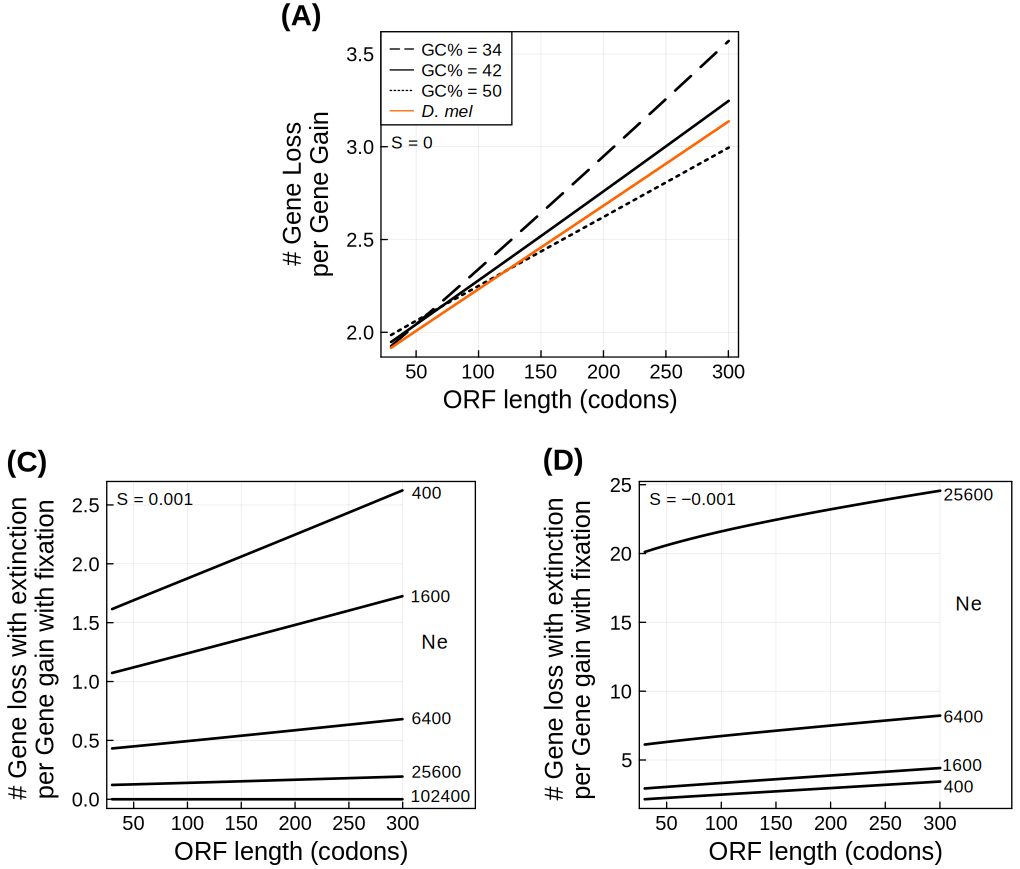
\includegraphics[scale=0.5]{Figures/pGainLossFix2.pdf}
\caption{Genes are more likely to be independently lost twice, than being born once. The vertical axis in all panels shows the number of independent gene loss events with extinction (\autoref{genelosseq}) that can occur relative to one gene gain event with fixation (\autoref{loglogratio}, \autoref{pFix}), under \textbf{(A)} no selection, \textbf{(B)} weak positive selection and \textbf{(C)} weak negative selection on the expression of the protein from a proto-gene. Horizontal axes show the number of codons in the ORF. Black lines in panel \textbf{(A)} denote the probability values estimated from overall GC content (34\%, 42\% and 50\%) and the orange line denotes the probability values estimated from trimer and hexamer frequencies in \textit{D. melanogaster} intergenic genome. In panels \textbf{(B)} and \textbf{(C)} we use the probabilitiy values from \textit{D. melanogaster} intergenic genome. $N_e$ denotes effective population size and $s$ denotes the selection co-efficient.}
\label{gainlossprob}
\vspace{1ex}
\hrule
\end{figure}

\cmnt{Natural selection and effective population size ($N_e$) determine the rate at which new genes spread in a population \citep{KimuraFix}. To understand the combined effect of mutations, and selection we calculated two fixation probabilities for populations consisting different number of diploid individuals. First is the probability that any one individual in a population gains a gene ($2N_e \times P_\textit{gene-gain}$), and this gene eventually spreads in entire the population via selection and population dynamics ($P_\textit{fix}$, \autoref{pFix}). The second probability describes the event that all individuals in a population have two copies of the proto-gene, one copy of the gene is lost in an individual ($2N_e \times P_\textit{gene-loss}$), and the gene eventually goes extinct from the entire population due to population dynamics ($P_\textit{ext}$, \autoref{pFix}). We calculated the log-log ratio of the two probabilities under three scenarios (\autoref{pFix}), wherein the gene provides no fitness advantage (neutral, $s=0$), the gene is marginally beneficial (positive, $s = 0.001$), and the gene is marginally deleterious (negative, $s = -0.001$). We note that gene gain and loss probabilities due to mutation are so small that it is unlikely that two or more individuals gain or lose a gene simultaneously. Under the neutral scenario, the probability of fixation of an allele is same as the probability of the mutation that gives rise to that allele (\hyperref[gainlossprob]{\autoref{gainlossprob}A}). Extinction of a marginally beneficial gene is more likely than its fixation only when populations are small or when the gene has a long ORF (\hyperref[gainlossprob]{\autoref{gainlossprob}B}). For example, a gene of any length is less likely to go extinct than it is fixed, in populations with at least 6400 individuals. Furthermore, a beneficial gene can be independently lost in more than two small populations with 400 individuals, only when it has more than 133 codons. When a gene is mildly deleterious, its is very likely to go extinct such that independent loss in more than two populations is more likely than its fixation in one population (\hyperref[gainlossprob]{\autoref{gainlossprob}C}). We further note that time to fixation of a rare allele (for example, a newly emerged protogene) would be much smaller \citep[$4N_e$ generations;][]{KimuraFix} than the time to gain ($10^{14}$ -- $10^{20}$ generations) or lose it ($10^{7}$ -- $10^{8}$ generations).}

Overall, our analysis suggests that a proto-gene expressed in only one population may not necessarily mean that it emerged for the first time in this population. \cmnt{This is also true for a model of gene emergence that requires a core promoter (TATA-box or Inr) for initiating transcription ({\color{blue} Figure S1}). 

Despite low probability of gene gain at one particular locus ($\sim 10^{-15}$ per generation), the overall rate of gene gain throughout the genome could be much higher. To this end we calculated the total gain rate of genes of any length, at any locus in \textit{D. melanogaster} intergenic genome. We found this rate to be $2.8\times 10^{-5}$ new genes per generation, that corresponds to approximately $7.5\times 10^{-5}$ new genes per year \citep[assuming \textit{D. melanogaster} generation time of two weeks;][]{drosophilaModelOrg}. We performed an analogous analysis on the rate of gain of new transcripts and found this rate to be 1.53 transcripts per year. This estimate is slightly higher than the rate of transcript gain predicted from \textit{D. melanogaster} population transcriptomics data \citep[0.13 -- 0.34;][]{AnnaPeteTranscripts}}. 

\subsection{Does \textit{de novo} gene emergence follow a preferred trajectory of events?}

For a proto-gene to emerge from a non-genic DNA sequence, both transcription and ORF need to emerge. That is, probability of gene emergence is equal to the product of probabilities of transcription gain and ORF gain. Thus it may appear that the order of the occurrence of these two events does not matter. However, gene emergence is much more likely when one of the two features already exists (\autoref{genegaineq}) and therefore it has two possible trajectories -- ORF emerges first (ORF-first) or transcription emerges first (RNA-first). Furthermore, emergence of an ORF is more likely when the proto-gene is already transcribed, and \textit{vice versa} (\autoref{rnaorfindependence}). To understand whether \textit{de novo} gene emergence has a preferred trajectory, we calculated two probabilities. First, the probability that an RNA exists and mutations cause a gain of an ORF but no disruption of transcription. This probability denotes the trajectory where RNA emerges first ($P_\textit{RNA-first}$, \autoref{rnafirsteq1}). 

\begin{equation}
P_\textit{RNA-first} = P_\textit{RNA-stay}\times P_\textit{ORF-gain \vline\ RNA}
\label{rnafirsteq1}
\end{equation}

The second probability ($P_\textit{ORF-first}$, \autoref{orffirsteq1}) that denotes the trajectory where ORF emerges first, is the probability that an ORF already exists and mutations cause a gain of transcription but do not disrupt the ORF.

\begin{equation}
P_\textit{ORF-first} = P_\textit{ORF-stay}\times P_\textit{RNA-gain \vline\ ORF}
\label{orffirsteq1}
\end{equation}


\begin{figure}[!t]
\centering
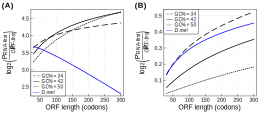
\includegraphics[scale=0.5]{Figures/whoisfirstX.pdf}
\caption{Proto-genes preferentially emerge RNA-first. The vertical axis shows the $\log_2$ transformed ratio of the probabilities of the RNA-first and the ORF-first trajectories, described as \textbf{(A)} a single-step process (Equations \ref{rnafirsteq1} \& \ref{orffirsteq1}) and \textbf{(B)} a two-step process (Equations \ref{rnafirsteq2} \& \ref{orffirsteq2}). A positive value suggests that RNA-first trajectory is more likely than ORF-first trajectory, and \textit{vice versa}. In both panels, the horizontal axis denotes the number of codons in the ORF. Black lines denote the probability values estimated from overall GC content (34\%, 42\% and 50\%) and the orange line denotes the probability values estimated from trimer and hexamer frequencies in \textit{D. melanogaster} intergenic genome.}
\label{whoisfirst}
\vspace{1ex}
\hrule
\end{figure}

\cmnt{We calculated the log-transformed ratio of $P_\textit{RNA-first}$ and $P_\textit{ORF-first}$, such that a positive value of the ratio would mean that ORF gain in an already transcribed DNA (RNA-first) is more likely than transcription gain for an untranscribed ORF (ORF-first). In other words, the RNA-first trajectory is more feasible. Likewise, a negative value of the ratio would suggest that the ORF-first trajectory is more feasible. We found that proto-genes with ORFs of all the investigated lengths, preferentially emerge RNA-first (\hyperref[whoisfirst]{\autoref{whoisfirst}A}). More specifically, the likelihood of the RNA-first trajectory relative to that of the ORF-first trajectory  increases with increasing ORF length. This is true for loci with three different values of GC content (34\%, 42\%, 50\%). However, our complementary analysis using DNA oligomer frequencies from \textit{D. melanogaster} intergenic genome shows that the likelihood of RNA-first trajectory relative to that of ORF-first trajectory, reduces with increasing ORF length. Nonetheless, RNA-first trajectory is still the more feasible trajectory of \textit{de novo} gene emergence. In a more stringent scenario of \textit{de novo} emergence, where a core promoter (TATA box or Inr) is necessary for transcription, proto-genes containing short ORFs can emerge ORF-first ({\color{blue}Figure S2})} 

A more stringent definition of the RNA-first trajectory would describe a two-step process. In the first step, an RNA emerges in an untranscribed region of DNA but an ORF does not emerge. In the second step an ORF emerges, while transcription stays intact (\autoref{rnafirsteq2}). Likewise, a ORF-first trajectory can be defined by a two-step probability. In the first step ORF emerges in an untranscribed DNA region, and in the second step transcription emerges, while the ORF remains intact (\autoref{orffirsteq2}).

\begin{align}
P_\textit{RNA-first}' & = \underbrace{P_\textit{RNA-gain} \times (1-P_\textit{ORF} -P_\textit{ORF-gain})}_\textit{first step} \times \underbrace{P_\textit{RNA-stay}\times P_\textit{ORF-gain \vline\ RNA}/(1-P_\textit{ORF})}_\textit{second step} \label{rnafirsteq2} \\[1em]
P_\textit{ORF-first}' & = \underbrace{P_\textit{ORF-gain} \times (1-P_\textit{RNA} -P_\textit{RNA-gain})}_\textit{first step} \times \underbrace{P_\textit{ORF-stay}\times P_\textit{RNA-gain \vline\ ORF}/(1-P_\textit{RNA})}_\textit{second step} \label{orffirsteq2}
\end{align}

\cmnt{Even with this stringent definition, \textit{de novo} emergence via the RNA-first trajectory is more probable than via the ORF-first trajectory (\hyperref[whoisfirst]{\autoref{whoisfirst}B}). For all the three GC-content values, as well the specific analysis with \textit{D. melanogaster} genome, the two-step RNA-first trajectory becomes increasingly more probable than the two-step ORF-first trajectory, with increasing ORF length.}


\subsection{Would extensive transcription loss suggest negative selection of toxic proteins?}


\begin{figure}[!b]
\centering
\hrule
\vspace{1ex}
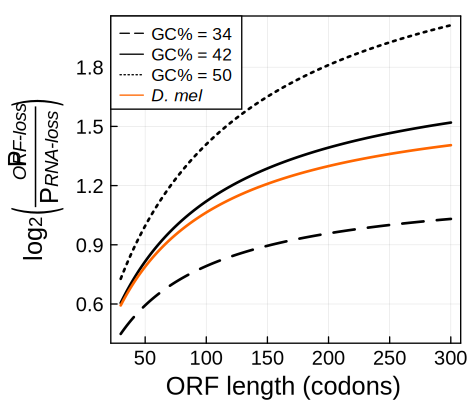
\includegraphics[scale=0.5]{Figures/pLoss_promoterlessX.pdf}
\caption{ORF loss in proto-genes is more probable than transcription loss. The horizontal axis denotes the number of codons in the ORF. The vertical axis shows the $\log_2$ transformed ratio of ORF loss and RNA loss probabilities, such that a positive value means ORF loss is more probable than RNA loss, and \textit{vice versa}. Black lines denote the probability values estimated from overall GC content (34\%, 42\% and 50\%) and the orange line denotes the probability values estimated from trimer and hexamer frequencies in \textit{D. melanogaster} intergenic genome.}
\label{lossprob}
\end{figure}

Proto-genes that do not provide any fitness benefit to an organism may not be fixed in populations via natural selection. These genes may be lost due to mutation pressure. Some newborn proto-genes can also encode toxic proteins, that may aggregate or interfere with physiology in some other way. These genes would thus be eliminated from the population genomes via negative selection. We note that an ORF is lost if the start codon is mutated, the stop codon is mutated to an amino acid encoding codon (non-stop mutation), or if an amino acid encoding codon is mutated to a stop codon (premature stop/non-sense mutation). However, it is likely that a non-stop mutation or a non-sense mutation, can still result in translation of a protein (extended or truncated, respectively). Furthermore, non-stop mutations can also lead to cellular toxicity \citep{nonstop}. Thus ORF loss does not ensure elimination of toxic proteins, which in turn suggests that transcription loss may more effectively inactivate the associated genes.

\cmnt{To understand which is the most probable mechanism of gene loss, we compared the probabilities of ORF loss ($P_\textit{ORF-loss}$) and transcription loss ($P_\textit{RNA-loss}$). We found that ORF loss is more probable than transcription loss, especially so when the ORFs are long (\hyperref[lossprob]{\autoref{lossprob}A}). If transcription is strictly dependent on a core promoter (TATA-box or Inr), small genes (30 codons) with low GC content ($>$34\%) can be preferentially lost by loss of transcription ({\color{blue} Figure S3}). When the organismal fitness is affected only by the protein product of a proto-gene, then both RNA loss and ORF loss would affect the fitness equally. Thus the likelihood of gene extinction through ORF loss or RNA loss depends solely on the probability of these events. 

Our analysis of gene loss mechanism considers the loss of one feature (for example transcription) without requiring the other feature to remain intact (for example the ORF). With more stringent analysis where we consider the loss of only one feature but not the other, we find a the that exclusive ORF loss is more likely than exclusive RNA loss ({\color{blue}Figure S5}). The difference between the likelihood of the two gene loss mechanisms is more remarkable when we consider exclusive loss of one feature.}

Overall, our analysis suggests widespread transcription loss may be indicative of a negative selection on protein expression.

\subsection{Does mutation bias shape protein composition?}

\begin{figure}[!t]
\centering
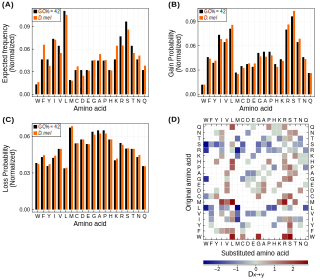
\includegraphics[scale=0.5]{Figures/proteinComposition.pdf}

\caption{Mutation bias and GC-content shape protein composition. Panels \textbf{(A)}, \textbf{(B)} and \textbf{(C)} show expected frequency, gain probability (\autoref{aagaineq}), and loss probability (\autoref{aalosseq}) for different amino acids (horizontal axes). The vertical axis in all these three subplots show the normalized values of these measures such that their sum over all amino acids is equal to one. Panel \textbf{(D)} shows the directionality (colored tiles, $\textit{D}_{x\to y}$, \autoref{directionality}) of the substitution from an amino acid (vertical axis) to another (horizontal axis). Positive values of $\textit{D}_{x\to y}$ are shown in shades of red, whereas negative values are shown in shades of blue. We only show substitutions that can be realized by a single nucleotide mutation but we include all possible nucleotide mutations in the directionality calculations for these substitutions. In all panels, amino acids are ordered based on their chemical similarity \citep{PMBEC}.}
\label{aafreq}

\vspace{1ex}
\hrule
\end{figure}

In previous sections, we showed that mutation bias affects the rate of \textit{de novo} gene emergence and loss. We next turned our attention to whether this bias affects the composition (and thereby the chemistry) of proteins encoded by proto-genes. To this end, we first asked if the expected frequency of different amino acids is uniform. For a GC-content of 42\% and with DNA trimer frequencies from \textit{D. melanogaster} intergenic genome, we found that it is not uniform. Amino acids like leucine (L) and serine (S) have a higher expected frequency than other amino acids. On the other hand, amino acids like methionine (M) and tryptophan (W) are less probable (\autoref{aafreq}{\color{blue}A}). This non-uniformity is to a great extent determined by number of degenerate codons for an amino acid. However, nucleotide composition also determines the frequency of an amino acid. For example, leucine, arginine and serine, all have six codons each. However, leucine is more likely to be encoded than serine in a random stretch of DNA, given a uniform GC-content of 42\% (\autoref{aafreq}{\color{blue}A}). The same is true for the frequencies of these amino acids estimated from the DNA trimer distribution. Overall, our analysis is roughly in agreement with many previous studies \citep{aasubOhta,aafreq3,aafreq4}. However, notable differences exist between our analysis and that of the previous studies because the latter primarily focused on characterized proteins and not random proto-gene derived protein sequences. 

Next, we aimed to find out if some amino acid substitutions are more probable than the others. To this end, we calculated the gain probability (\autoref{aagaineq}) for every amino acid. Specifically for every amino acid $x$, we calculated the average probability that it substitutes any of the other nineteen amino acids, due to mutations. More precisely, the total probability that an amino acid $y$ will mutate to an amino acid $x$ is the product of the expected frequency of amino acid $y$ ($P_y$), and the substitution rate from $x$ to $y$ ($\mu_{y\to x}$). The gain probability for an amino acid $x$ is then defined as:

\begin{equation}
G_x = \sum_{b \neq a} P_y \times \mu_{y\to x}
\label{aagaineq}
\end{equation}

We found that amino acid gain probabilities were also non-uniform across different amino acids (\autoref{aafreq}{\color{blue}B}) but they had a strong positive correlation with the expected frequency (GC = 42\%, Pearson $\rho = 0.955, P<10^{-10}$; \textit{D. melanogaster} trimer frequencies, Pearson $\rho = 0.841, P<10^{-10}$).

Next, we calculated how easily is an amino acid mutated to any other amino acid. Specifically, the conditional loss probability for an amino acid ($L_x$), given the amino acid already exists, is defined as:

\begin{equation}
L_x = \sum_{x \neq y} \mu_{x\to y}
\label{aalosseq}
\end{equation}


The loss probability was also not uniformly distributed (\autoref{aafreq}{\color{blue}C}) but it did not significantly correlate with the expected frequency of the amino acids (GC = 42\%, Pearson $\rho = -0.255, P = 0.2818$; \textit{D. melanogaster} trimer frequencies, Pearson $\rho = -0.356, P=0.1232$).

Next, we investigated if some amino acid substitutions are more common than the others. As expected, amino acid substitutions that require more than one nucleotide change were much less probable than those needing just a single nucleotide change. Therefore, we focused our analysis on amino acid substitutions whose total probabilities were more than that of a double nucleotide mutation (note that this procedure identifies amino acid substitutions that are possible via single nucleotide mutations but it does not exclude multinucleotide mutations from the calculation of amino acid substitution probabilities). Although single nucleotide mutations are more probable than double mutations, the different single mutations do not occur at the same rate due to mutation rate bias. Thus an amino acid substitution (for example K$\to$E) may not be as likely to occur as the reverse substitution (E$\to$K). That is substitutions between a pair of amino acids may have a directionality. Although many previous studies have explored the likelihood of different amino acid substitutions \citep{aasubOhta,PAM,blosum,submat92,submat92j,submat01,submat05,submat07,submat08}, none to our knowledge have focused primarily on the directionality of these substitutions. To verify if such a directionality exists, we calculated the log transformed ratio of forward and reverse substitution probability, $D_{x\to y}$, for every pair of amino acids, $x$ and $y$. A positive value of $D_{x\to y}$ means that $x$ to $y$ substitution is more likely than $y$ to $x$ substitution, and \textit{vice versa}.

\begin{equation}
\textit{D}_{x\to y} = \log_2\left(\frac{\mu_{x\to y}}{\mu_{y\to x}}\right)
\label{directionality}
\end{equation}

As we mentioned in the previous paragraph, we restricted this analysis to substitutions that can be achieved via single nucleotide mutations. We found that most substitutions indeed had a preferred direction ($\textit{D}_{xy} \neq 0$,  \autoref{aafreq}{\color{blue}D}). The median absolute value of $\textit{D}_{xy}$ was 0.905 and the maximum value was 2.836. That is, in 38 out of 75 amino acid pairs we analysed, one direction of substitution was at least 1.87 times more probable than the other. For example, E$\to$K substitution is 1.8 times more probable than K$\to$E substitution. This may appear as a small number but many such unidirectional substitutions occurring in an evolving protein could indicate a directional selection. \cmnt{We note that that actual frequencies of specific substitutions depend on the initial distribution of different codons in the ORF sequence.}


A previous study found that mutations that cause hydrophobic amino acids to appear on protein surfaces, can lead to evolution of protein dimers \citep{hydrophobicRatchet}. The authors also suggested that such an evolutionary process may be widespread because mutation bias tends to facilitate emergence of hydrophobic amino acids. They based this argument on another study that estimated mutation rate bias in bacteria \citep{bacteriaMutbias}. The authors \citep{hydrophobicRatchet} further suggested that hydrophobic amino acids are more frequently found in random protein sequences. 

We asked if our model also makes similar predictions. To this end, we first calculated the percentage of amino acids in a protein sequence that are expected to be hydrophobic. A popular hydrophobicity scale of amino acids is based on solubility of an amino acid in water or ethanol \citep{hydropathy}. However, this scale does not classify tryptophan as a hydrophobic amino acid. Another hydrophobicity scale estimated by a different study \citep{WWhydropathy} is more biologically realistic and is based on rates of transfer of different amino acids between water and a hydrophobic medium. This study analysed two hydrophobic media -- a lipid bilayer and octanol, and also considered the effect of peptide bonds in the calculations. Therefore we used the hydrophobicity scale by \cite{WWhydropathy} for classifying amino acids such that hydrophobic amino acids have a negative free energy change of transfer from water to hydrophobic media. Conversely, a hydrophilic amino acid would have a positive value of the free energy change. Based the octanol hydrophobicity scale, we classified the following amino acids as hydrophobic -- cysteine (C), phenylalanine (F), isoleucine (I), leucine (L), methionine (M), valine (V), tryptophan (W) and tyrosine (Y). With the lipid bilayer hydrophobicity scale, valine is not classified as hydrophobic, possibly because it does not integrate well in the bilayer. Therefore we used the octanol scale for our calculations.

We found that $\sim$40\% of amino acids in a protein sequence are expected to be hydrophobic (with a GC-content of 42\% as well as with \textit{D. melanogaster} trimer distribution). This finding is broadly in agreement with the previous study \citep{hydrophobicRatchet}. We note that cytosolic proteins may require more than 42\% of their constituent amino acids to be hydrophobic, in order to fold efficiently \citep{Dill1985}. Next, we asked if a protein sequence in general tends to be hydrophobic. Specifically, we calculated expected hydrophobicity ($\bar{\alpha}$, \autoref{expHydropathy}) of a protein sequence, based on expected frequency of different amino acids ($P_x$, \autoref{aafreq}) and their hydrophobicity values ($\alpha_x$). 

\begin{equation}
\bar{\alpha} = \sum_{x} P_x \alpha_x
\label{expHydropathy}
\end{equation}


We found that the expected hydropathy is higher than zero (0.38 with GC\% = 42; 0.36 with \textit{D. melanogaster} trimer frequencies), which suggests that random protein sequences are not on an average, hydrophobic.
 
To find out if random mutations indeed cause hydrobphobic amino acids to occur in protein sequences, we calculated the probability that any mutation substitutes a non-hydrophobic amino acid with a hydrophobic amino acid ($P_{\alpha\textit{-gain}}$, \autoref{alphagain}). Likewise, we calculated the probability that any mutation causes a hydrophobic to non-hydrophobic amino acid substitution ($P_{\alpha\textit{-loss}}$, \autoref{alphaloss}).  

\begin{align}
P_{\alpha\textit{-gain}} & = \sum_{\genfrac{}{}{0pt}{1}{x}{\,|\,\alpha_x>0}} \sum_{\genfrac{}{}{0pt}{1}{y}{\,|\,\alpha_y \geq 0}} P_y \times \mu_{y\to x}\label{alphagain}\\[1em]
%
P_{\alpha\textit{-loss}} &= \sum_{\genfrac{}{}{0pt}{1}{x}{\,|\,\alpha_x>0}} \sum_{\genfrac{}{}{0pt}{1}{y}{\,|\,\alpha_y \geq 0}} P_x \times \mu_{x\to y}\label{alphaloss}
\end{align}

Next, we calculated the ratio of $P_{\alpha\textit{-gain}}$ and $P_{\alpha\textit{-loss}}$, and found that it is slightly more than 1 (1.114 with GC\% = 42; 1.015 with \textit{D. melanogaster} trimer frequencies). This suggests that gain of a hydrophobic amino acid is slightly more probable than its loss. We performed a complementary analysis where we calculated the average change in hydrophobicity due to any random mutation ($\bar{\Delta\alpha}$), defined by:

\begin{equation}
\bar{\Delta\alpha} = \frac{\displaystyle\sum_{x} \sum_{y} \mu_{x\to y} \times (\alpha_y - \alpha_x)}{\displaystyle\sum_{x} \sum_{y} \mu_{x\to y}}
\end{equation}

We found the average change in hydrophobicity to be slightly less than zero ($-0.0798$), which suggests that on an average mutations cause a very small increase in hydrophobicity. We reiterate that hydrophobic amino acids have a negative value hydrophobicity and thus a negative change in hydrophobicity also denotes a shift towards a more hydrophobic protein. To focus exclusively on non-hydrophobic to hydrophobic amino acid substitutions, we excluded amino acid pairs where both amino acids are either hydrophobic or are non-hydrophobic. That is, we only analysed pairs of amino acids that have opposite signs of hydrophobicity. With this focused analysis, we find that the average change in hydrophobicity is comparable ($-0.0793$). For both the analyses, we note that the actual change in hydrophobicity will depend on the composition of the ancestral protein sequence.

Overall our analyses show that random mutations may preferentially cause hydrophobic amino acids to accumulate in protein sequence but this effect may be very small.

\section{Discussion} 

In this work, we addressed some fundamental questions about \textit{de novo} emergence of protogenes. Broadly, we asked how quickly these genes can emerge and be lost, whether their birth and death has a preferred trajectory of mutational events, and how the composition of their protein sequence is determined. To this end, we developed mathematical models and used them to address specific questions. These models are based on mutation probability and mutation rate bias, and represent neutral evolution where DNA sequences are not evolving under natural selection. Thus our models provide an opportunity to test the alternative hypothesis that some proto-genes are evolving under selection.

We show that when a protein product of a proto-gene doesn't affect organismal fitness, the gene can be lost much more rapidly than they are gained, such that it can be independently lost two to three times in the time required for it to emerge (\hyperref[gainlossprob]{\autoref{gainlossprob}A}). In a hypothetical case, a proto-gene may be present in a population (A) but is absent in two other geographically isolated populations (B and C). Two evolutionary scenarios could explain this observation. In the first scenario, the proto-gene simply emerged for the first time in population A. The second scenario posits that the proto-gene was present in the ancestral population but was lost in both population B and population C. Our models suggest that the second scenario is more likely than is assumed. \cmnt{This inference can be further extended to the level of closely related species where the divergence times are relatively shorter than the timescale of multiple gain and loss events within a lineage}. Future phylogenetic studies on proto-genes should consider this finding for inferring the dynamics of gene gain and loss. \cmnt{Proto-genes that encode proteins that are beneficial to an organism's fitness are likely to be protected in the genome against gene loss \citep{Lee2019}. Our models indeed show that loss of even moderately beneficial genes is unlikely in large populations (\hyperref[gainlossprob]{\autoref{gainlossprob}B})}.

Within the limitations of our model assumptions, we answer the long standing question of which trajectory of mutational events leads to \textit{de novo} emergence. That is, whether ORF emerges first or transcription emerges first \citep{EBB-F1000}. We show that, in the absence of selection, genes are likely to emerge in existing transcripts (transcription emerges first, \autoref{whoisfirst}). Long non-coding RNAs may be a potential source of proto-genes but this evolutionary process may be constrained by a different set of factors. A previous study has shown that new transcripts frequently arise in regions overlapping existing genes. These new transcripts can harbor ORFs which in turn leads to \textit{de novo} gene emergence \citep{albaYeastdenovo}. This is an example of RNA-first trajectory. However, the ORFs present in these genes may be under indirect selection pressure that acts on the overlapping gene sequences. Therefore, they may be less frequently mutated or lost.

Although our model is based on the assumption of neutral evolution, one can speculate the effects of positive selection on the proto-gene. For example, if an ORF encodes a protein that is beneficial to the organism, then selection would cause the fixation of the gene as soon as the it emerges via RNA-first trajectory. On the other hand, the selection would have no effect on an ORF that is not transcribed, as long as it is does not harbor a functional DNA sequence (such as regulatory elements), and is not under indirect selection (for example, if it overlaps with an existing gene). The ORF may mutate before transcription emerges and the corresponding mutated protein may not be beneficial anymore. Thus positive selection may further increase the likelihood of the RNA-first trajectory.

We show that transcription loss is less likely than the loss of long ORFs (\autoref{lossprob}). However, it may be difficult to find direct evidence for such a phenomenon. Specifically, it is difficult to infer from data if transcription was lost or never emerged. If the protein encoded by an ORF is indeed toxic, it would be silenced or purged rapidly in microevolutionary time scales. One way of inferring negative selection from transcription loss may involve correlation of ORF sequence variation and transcription status. Mutations within an ORF sequence are much more probable than mutations that disrupt transcription or an ORF. This is so because the entire ORF sequence can have a higher number of mutable sites than a promoter. If an ORF variant is untranscribed in many populations (species or taxa), it is possibly toxic.  

A large volume of work exists on the likelihood of amino acid substitutions and many of these models are widely used in phylogenetics studies \citep{aasubOhta,PAM,blosum,submat92,submat92j,submat01,submat05,submat07,submat08}. However, commonly used amino acid substitution models such as PAM and BLOSUM \citep{PAM,blosum} do not focus on directionality of mutations (the substitution matrices are symmetric). Our aim was to highlight how proteins can evolve under mutation pressure and that mutation bias causes some substitutions to occur more frequently than the others. Furthermore, we do not base our substitution probability calculations on known protein sequences but rather on random protein sequences that are more likely to to be encoded in proto-genes. Using our models, we show that for a pair of amino acids, one direction of substitution can be significantly more likely than the other. If a substitution occurs more frequently than it is expected to occur in our neutral model, then directional evolution can be a possible explanation for the observation. We also show that random mutations can lead to a small increase in a protein's hydrophobicity. Hydrophobic amino acids can facilitate folding \citep{Dill1985}, but can also cause proteins to aggregate \citep{hydrophobicRatchet}. Thus the effect of hydrophobicity increasing mutations on a protein's stability and toxicity, is dependent on where they occur in the protein structure.

Like all theoretical models, our models are not without limitations. First, we assume that nucleotides are uniformly distributed according to GC-content. This is not true as nucleotide composition can vary significantly across the genome. \cmnt{Since our model primarily focuses on gene emergence at one locus, it can be used to predict evolutionary probabilities for different genomic loci. Furthermore, several predictions of our models are not qualitatively affected by GC-content. More realistic nucleotide composition distribution estimated from \textit{D. melanogaster} intergenic sequences, also qualitatively agree with GC-content based predictions. Thus, most predictions are qualitatively robust to small differences in parameters. Second, in our models, we assumed uniform mutation rate throughout the genome. However, recent studies have shown that mutation rates are also not uniform across the genome, and can vary significantly \citep{mutbiasArabidopsis}}. Our models can be adapted to investigate specific genomic loci, where estimates of the local nucleotide composition and mutation rate can more accurately determine the \textit{de novo} gene evolution in these loci. Third, our models are based on parameters such as mutation rate and mutation bias, which we obtained from published data on human and \textit{D.melanogaster} genomes \citep{humanmutrate,drosophilamutrate}. The accuracy of the models' prediction will depend on the accuracy of parameters. However, mutation rate itself only determines the values of different probabilities. Our results, which are based on probability ratios, will not significantly change with a different value of mutation rate. Mutation bias may have more significant effect on the predictions than mutation rate. Existing data suggest that different species have a different spectrum of mutations \citep{joshmutbias}, especially for species that are highly distant from each other. Thus our inferences based on our chosen parameters will not universally apply to all species. Fourth, we assume that occurrence of a point mutation is independent of another mutation. This is not the case for tandem mutations, where multinucleotide mutations occur more frequently than their expected frequency under the assumption of mutational independence \citep{MNM}. Fourth, we did not specifically model the effect of many regulatory sequence features such as enhancers, transcription factor binding sites, 5' and 3' untranslated regions, and Kozak consensus sequence, that can influence the evolution of proto-genes. For example \textit{de novo} emergence is very likely to occur near enhancers \citep{PacoEnhancers}. \cmnt{To model this phenomenon in our analyses, we assumed that DNA loci feasible for transcript emergence are close to known \textit{cis-} regulatory elements \citep{RedFly2005,RedFly2007,RedFly2010,RedFly2018,RedFly2022}. Specifically, we assumed that transcription can be initiated at a probability that is equal to the proportion of such regulatory elements in the intergenic genome. This is a rough estimate but it can be updated when more specific data becomes available. For example, ATAC-seq data can provide reliable estimates of nucleosome depleted regions, that can act as transcription initiation sites \citep{ATAC-seq}. This analysis can be supplemented with data from techniques like native elongating transcript sequencing \citep[NET-seq;][]{NET-seq} and global run-on sequencing \citep[GRO-seq;][]{GRO-seq}, that can detect nascent transcripts.} Our modeling framework also allows incorporation of any number of sequence features in the calculations as long as their sequences can be defined (\autoref{methfeatures}). Finally, we ignore insertions, deletions and transpositions as mechanisms of mutation. Insertions and deletions (indels) are reported to be less frequent than substitutions \citep{drosophilamutrate}, and both indels and transpositions cause larger sequence alterations than point mutations. Our modeling methodology also allows incorporation of these mechanisms as a source of mutations. 

A famous aphorism about theoretical models says ``all models are wrong but some are useful'' \citep{GEBox}. Our models are not an exception. They may not be 100\% accurate but they make useful predictions that can lead to a more focused experimental validation. \cmnt{Many of our predictions are qualitatively robust to small parameter changes. Some predictions are also in agreement with experimental data. For example, our prediction of transcript gain rate is only slightly inflated than the estimated rates using an empirical analysis of \textit{D. melanogaster} populations \citep{AnnaPeteTranscripts}. This difference could have possibly resulted from our relaxed requirements for a promoter, or other unknown factors that may have affected population evolution \citep[for example, the actual effective population size and environmental conditions;][]{dmel3decades}. When supplemented with experimental data analysis our models can be made more complex to accommodate diverse molecular mechanisms driving gene evolution, and can provide more accurate predictions.} Therefore our work opens up an opportunity for theoretical and computational biologists to design analyses using our modeling framework, that more accurately describe their system of interest.

\section{Materials and Methods}

\subsection{Mutation probabilities}

\begin{table}[H]
\centering
\begin{tabular}{c c}
\toprule
\textbf{Substitution} & Probability($\mu$) \\\midrule
\texttt{A:T}$\to$\texttt{T:A} & 0.056 \\\midrule
\texttt{A:T}$\to$\texttt{G:C} & 0.243 \\\midrule
\texttt{A:T}$\to$\texttt{C:G} & 0.074 \\\midrule
\texttt{G:C}$\to$\texttt{A:T} & 0.483 \\\midrule
\texttt{G:C}$\to$\texttt{T:A} & 0.075 \\\midrule
\texttt{G:C}$\to$\texttt{C:G} & 0.069 \\\bottomrule
\end{tabular}
\caption{Mutation bias probabilities for different nucleotide mutations. \texttt{A:T} denotes an \texttt{A}-\texttt{T} base pair in a double stranded DNA. Thus \texttt{A}$\to$\texttt{G} mutation on one DNA strand would cause a \texttt{T}$\to$\texttt{C} mutation on the complementary strand. We describe the other mutations in the same way.}
\label{mutbias}
\end{table}

We calculated nucleotide substitution probabilities based on mutation rate and mutation rate bias data. Specifically, we  used a mutation rate ($\lambda$) of $7.8\times10^{-9}$ mutations per nucleotide position per generation \citep{drosophilamutrate}. We derived our mutation bias parameters from two published studies, the first on \textit{Drosophila melanogaster} \citep{drosophilamutrate}, and the second on humans \citep{humanmutrate}. \autoref{mutbias} shows the exact values of mutation bias probabilities that we used in this study.



\subsection{Probabilities of finding, gaining, and losing a DNA sequence}
\label{methbasic}

\subsubsection{Probability of finding a DNA sequence}
\label{methprob}

We calculated the probability of finding a DNA sequence based on global nucleotide frequency distributions, given by the GC-content. Specifically, the probability of finding either a \texttt{G} or a \texttt{C} is: 

$$S = \frac{0.5\times\text{GC\%}}{100}$$

The probability of finding an \texttt{A} or a \texttt{T} is: $W = 0.5 - S$. Using these values, we calculated the probability of finding a DNA sequence motif by chance. For example, the probability of finding the sequence \texttt{ATG} would be: $W\times W \times S$.

\cmnt{We also estimated the probability of finding specific DNA sequences in a reference genome. Specifically, we calculated the frequencies of all 64 trimers and all 4096 hexamers in the genomic regions of \textit{D. melanogaster} that exist in open chromatin, and do not contain any known genes or regulatory elements (see \autoref{methRNA})}.

\subsubsection{Probability of gaining a DNA sequence}
\label{methgain}

We calculated the probability of gaining a DNA sequence due to mutations using GC-content, mutation rate and mutation bias. Specifically, we calculated the probability that a DNA sequence does not exist, and it emerges due to specific nucleotide mutations. More precisely, this probability is the product of two other probabilities. The first is the probability of finding a DNA sequence ($x$) that is not the sequence of interest. The second probability is that this sequence $x$ mutates to the sequence of interest. To explain this calculation better, we use the example of \texttt{CTA} mutating to \texttt{ATG}. The first probability, that is the probability of finding \texttt{CTA} by chance is $SW^2$. \texttt{CTA} mutates to \texttt{ATG} via two nucleotide mutations (\texttt{C}$\to$\texttt{A} and \texttt{A}$\to$\texttt{G}). Thus the probability of this DNA change would be the probability of two nucleotide mutations ($\lambda^2$) multiplied by two mutation bias probabilities (\texttt{G:C}$\to$\texttt{T:A} and \texttt{A:T}$\to$\texttt{G:C}). Overall, the chance of \texttt{CTA} mutating to \texttt{ATG} would be:

$$SW^2 \times \lambda^2 \times \mu_{\texttt{G:C}\to\texttt{T:A}} \times \mu_{\texttt{A:T}\to\texttt{G:C}}$$

Next, we calculated the probability that every nucleotide triplet that is not \texttt{ATG}, mutates to \texttt{ATG}. This can happen via one, two, or three nucleotide mutations. The sum of all these mutation probabilities is the probability of \texttt{ATG} gain.

Using the same principle we calculated the gain probability of any DNA sequence motif (of any length or composition). We excluded insertions and deletions as a mechanism of gain of small DNA sequences that we analysed in this study. 


\subsubsection{Probability of losing a DNA sequence}

We calculated the loss of a DNA sequence motif using the same principle we used for calculating gain probabilities. However, we defined loss probability as a conditional probability, that is we assume that the DNA sequence of interest already exists in the genome. For example, the loss probability of a specific \texttt{ATG} sequence would be the sum of probabilities of \texttt{ATG} mutating to any of the other 63 nucleotide triplets (via one, two, or three nucleotide mutations). We use conditional loss probabilities by default, because usually one is interested in finding out how quickly an existing DNA sequence can erode.

We used this method to calculate the loss probability of any DNA sequence motif, and we excluded insertions and deletions from this calculation.

\subsection{Probabilities of finding, gaining, and losing DNA features}
\label{methfeatures}

Usually, a specific function is encoded in DNA by several DNA sequences. For example, translation stop is encoded by three codons (\texttt{TGA}, \texttt{TAG}, \texttt{TAA}). We use the term DNA features to mean a set of DNA sequences that are associated with the same function. For every such DNA feature set, there is a complementary set of non-features, that is DNA sequences that are not associated with the feature's function. For example, the non-feature set of stop codons would be all the other 61 codons. 

The probability that a DNA feature exists, is the sum of probabilities of every DNA sequence in that set (\autoref{methprob}).

The probability that a DNA feature is gained via mutations, is the sum of probabilities of every non-feature sequence mutating to any feature sequence. If $F$ denotes the feature set, and $\mu_{y\to x}$ denotes the probability of a DNA sequence $y$ mutating to a DNA sequence $x$ (see \autoref{methgain}), then:

\begin{equation}
P_\textit{feature-gain} = \sum_{x \in F} \sum_{y \notin F} P_y \times \mu_{y\to x}
\end{equation}

The probability that a DNA feature is lost via mutations is a conditional probability that given a feature exists, it mutates to any of the non-feature sequences. 

\begin{equation}
P_\textit{feature-loss} = \frac{\displaystyle\sum_{x \in F} \sum_{y \notin F} P_x \times \mu_{x\to y}}{\displaystyle\sum_{x \in F} P_x}
\end{equation}

Because a feature set usually has many DNA sequences, a mutation can change a feature sequence such that the resulting sequence is also a part of the feature set. Thus we defined the probability ($P_\textit{feature-stay}$) that a feature does not erode because of mutations. Specifically, it is the sum of two probabilities. First is the probability that no mutation occurs in the DNA sequence ($P_0$), and the second probability describes the event where the mutated sequence remains a part of the feature set.

\begin{equation}
P_\textit{feature-stay} = P_0 + \sum_{x \in F} \sum_{\genfrac{}{}{0pt}{1}{y \in F}{y\neq x}} \mu_{x\to y}
\end{equation}


The probability that no mutation occurs ($P_0$) in a DNA sequence of length $k$ is described by Poisson distribution. 

$$P_0 = 1-e^{-k\lambda}$$

Because the mutation rate is biased (\autoref{mutbias}), the probability that no mutation occurs in a DNA sequence depends on its composition. 

The probability that an \texttt{A} or a \texttt{T} mutates ($\lambda_\texttt{AT}$), is thus described as:

$$\lambda_\texttt{AT} = 2\times\lambda\times(\mu_{\texttt{A:T}\to\texttt{T:A}} + \mu_{\texttt{A:T}\to\texttt{G:C}} + \mu_{\texttt{A:T}\to\texttt{C:G}})$$

Likewise, the probability that a \texttt{G} or a \texttt{C} mutates ($\lambda_\texttt{GC}$) is: 

\vspace{-1ex}

$$\lambda_\texttt{GC} = 2\times\lambda\times(\mu_{\texttt{G:C}\to\texttt{A:T}} + \mu_{\texttt{G:C}\to\texttt{T:A}} + \mu_{\texttt{G:C}\to\texttt{C:G}})$$

(Note that the general mutation rate, $\lambda$, is an average of $\lambda_\texttt{AT}$ and $\lambda_\texttt{GC}$.)

\vspace{1\baselineskip}

Thus the probability that a sequence of length $k$, containing $m$ number of \texttt{A} and \texttt{T}, does not mutate is:

\vspace{-1ex}

$$P_0 = (1-e^{-m\lambda_\texttt{AT}})\times(1-e^{-(k-m)\lambda_\texttt{GC}})$$


\cmnt{We also calculated all the above-defined probabilities ($P_\textit{feature-gain}$, $P_\textit{feature-loss}$ and $ P_\textit{feature-stay}$), using DNA trimer and hexamer frequencies from \textit{D. melanogaster}. In this case the probability of finding a nucleotide sequence depends on the trimer/hexamer distributions instead of GC-content, but the probability of mutational changes are only dependent on mutation bias. Trimers and hexamers would contain codons and polyA signals, respectively.}



\subsection{Probabilities of finding, gaining, and losing an ORF}

\label{methORF}

\subsubsection{Probability of finding an ORF}

A reading frame is a nucleotide sequence with a length that is a multiple of three. A reading frame that begins with a start codon (\texttt{ATG}), and ends with one of the three stop codons (\texttt{TAG}, \texttt{TGA}, \texttt{TAA}) is an open reading frame (ORF). This necessarily means that there are no stop codons within the sequence. Thus the probability of finding an ORF containing $k$ codons including start and stop codons ($P_\textit{ORF}$) is: 

\begin{equation}
P_\textit{ORF}(k) = P_\textit{ATG} \times P_\textit{stop} \times (1 - P_\textit{stop})^{k-2}
\label{eqorfprob}
\end{equation}

Here, $P_\textit{ATG}$ and $P_\textit{stop}$ are the probabilities of finding a start codon, and a stop codon by chance, respectively.

\subsubsection{Probability of gaining an ORF}

As we defined in the previous section, an ORF has three requirements (start codon, stop codon, and no premature stop codon in the sequence). Thus an ORF can emerge due to mutations via three mechanisms. In each of these mechanisms, one requirement is initially absent whereas the other two are present. Then mutations cause the missing requirement to emerge while not disrupting the other two requirements. More specifically, the ORF can be gained via the following three mechanisms:
\begin{enumerate}
\item Gain of a start codon ($P_\textit{ATG-gain}$) while a stop codon continues to exist at the end of a reading frame ($P_\textit{stop-stay}$), and there is no emergence of stop codon within the reading frame ($1- P_\textit{stop} - P_\textit{stop-gain}$).
\item Gain of a stop codon ($P_\textit{stop-gain}$), while a start codon continues to exist at the beginning of a reading frame ($P_\textit{ATG-stay}$), and there is no emergence of stop codon within the reading frame.
\item Loss of a premature stop codon, at any of the $k-2$ codon positions within the reading frame ($P_\textit{stop-gain}$). At the same time start and stop codons remain undisrupted by mutations, and no stop codon emerges at any of the other $k-3$ positions.
\end{enumerate} 

Thus we define the probability of ORF gain ($P_\textit{ORF-gain}$) as:

\begin{align}
P_\textit{ORF-gain}(k) & = \quad P_\textit{ATG-gain}\times P_\textit{stop-stay} \times (1- P_\textit{stop} - P_\textit{stop-gain})^{k-2} \nonumber \\[1pt]
& \quad + P_\textit{ATG-stay}\times P_\textit{stop-gain} \times (1- P_\textit{stop} - P_\textit{stop-gain})^{k-2} \nonumber \\[1pt]
& \quad + P_\textit{ATG-stay}\times P_\textit{stop-stay} \times P_\textit{stop-loss}\times(k-2) \times (1- P_\textit{stop} - P_\textit{stop-gain})^{k-3} 
\label{eqorfgain}
\end{align}

\subsubsection{Probability of ORF loss}

ORF can be lost when any of its three requirements are lost. We thus define the conditional probability of ORF loss as:

\begin{equation}
P_\textit{ORF-loss}(k) = P_\textit{ATG-loss} + P_\textit{stop-loss} + (k-2)\times \frac{P_\textit{stop-gain}}{1-P_\textit{stop}}
\label{eqorfloss}
\end{equation}

The last term in this equation describes the conditional probability of stop-gain, given the assumption that no stop codon exists within the ORF.

\subsubsection{Probability that ORF remains intact}

We assumed that an ORF of a certain length remains intact if none of the necessary features are lost. However, the ORF sequence can mutate to cause non-synonymous changes in the translated protein sequence. This condition applies to all the three ORF probabilities described above. We define the probability that an ORF remains intact ($P_\textit{ORF-stay}$) as:

\begin{equation}
P_\textit{ORF-stay}(k) = P_\textit{ATG-stay} \times P_\textit{stop-stay} \times (1 - P_\textit{stop} - P_\textit{stop-gain})^{k-2}
\label{eqorfstay}
\end{equation}

\subsection{Probabilities of finding, gaining, and losing transcription}

\label{methRNA}

\subsubsection{Probability of transcription}

\cmnt{In this study we defined a transcription model that is not dependent on specific promoter sequences. Instead we defined a probability that transcription is initiated at a genomic locus. To this end, we first extracted the genomic coordinates of intergenic sequences in \textit{D. melanogaster} genome \citep[release 6.49, FlyBase;][]{flybase}. Using the data on the genomic locations of open chromatin in \textit{D. melanogaster} \citep{dmel_Chromatin}, we obtained open chromatin regions within intergenic genome. Next, we calculated the fraction of this open-intergenic genome occupied by \textit{cis-} regulatory elements \citep{RedFly2005,RedFly2007,RedFly2010,RedFly2018,RedFly2022}. A significant proportion of these elements include enhancers. Enhancers, that can promote transcription in their neighboring genomic regions \citep{enhancers}, are also known to promote \textit{de novo} gene emergence \citep{PacoEnhancers}. Thus we reasoned that proportion of \textit{cis-} regulatory elements in open intergenic chromatin would roughly approximate the likelihood of transcription initiation ($P_\textit{RNAinit}$). We do not model the exact sequences because data is not yet available on exact sequence requirements and mutational robustness of enhancers and other \textit{cis-} regulatory elements. Thus poly-A signal is the primary sequence determinant of transcription probabilities. Relatedly, open intergenic chromatin regions, that are not interrupted by \textit{cis-} regulatory elements are the potential sites for \textit{de novo} gene emergence.

A poly-A signal marks the end of a transcript. The transcribed DNA region should thus have only one poly-A signal at its end.} A transcribed DNA of length $l$ nucleotides, contains $l-5$ hexamers (6nt long sequences). Each of these hexamers can be a poly-A signal with a probability, $P_\textit{polyA}$. Probability that none of these hexamers is a poly-A signal is $(1-P_\textit{polyA})^{l-5}$. Since we focus on protein coding genes in this work, we describe the length of transcript in terms of the length of protein it can encode. Assuming that untranslated regions have no effect on protein synthesis, the length of a transcript in number of nucleotides should be at least three times the length of the encoded protein in number of amino acids. Thus the probability that a DNA region produces a transcript that can harbor an ORF with $k$ codons ($P_\textit{RNA}(k)$) is:

\begin{equation}
P_\textit{RNA}(k) = P_\textit{RNAinit} \times P_\textit{polyA} \times (1-P_\textit{polyA})^{3k-5}
\label{eqrnaprob}
\end{equation}

\subsubsection{Probability of gaining transcription}

\cmnt{As we mentioned in the previous section, two requirements need to be met to produce a transcript of any given length. First, a poly-A signal needs to be present at the end of the DNA region to be transcribed, and second, no poly-A signal should exist within this DNA region. Transcription can be gained if one of these requirements are already met and the third required feature emerges due to mutations. At the same time mutations should not destroy the existing features. It is possible that both the required features are missing and they emerge simultaneously due to mutations. However such an event is highly improbable. Thus transcription gain can occur via two mechanisms. In the first mechanism a poly-A signal is gained at the end of a sequence ($P_\textit{polyA-gain}$), while no poly-A sites are present at any $l-5$ (or $3k-5$) sites within the sequence, and none emerge ($P_\textit{nopolyA-stay} = 1 - P_\textit{polyA} - P_\textit{polyA-gain}$). In the second mechanism, a poly-A signal is present at the end of the sequence, and is not lost due to mutations. Meanwhile, one poly-A signal at any of the $3k-5$ sites within the sequence is lost ($P_\textit{polyA-loss}$), whereas the other $3k-6$ sites do not encode a poly-A signal and continue to remain so.

The combined probability of these two transcription gain mechanism is defined as:

\begin{equation}
P_\textit{RNA-gain}(k) = P_\textit{RNAinit} \times \begin{pmatrix}
P_\textit{polyA-gain}\times (P_\textit{nopolyA-stay})^{3k-5} \\[1em]
 +\  P_\textit{polyA-stay}\times (P_\textit{nopolyA-stay})^{3k-5} \times (3k-6) \times P_\textit{polyA-loss}
\end{pmatrix}  
\label{eqrnagain}
\end{equation}

\subsubsection{Probability of losing transcription}

Transcription is lost when either the poly-A signal is lost or if one is gained within the transcribed sequence. The probability of transcription loss ($P_\textit{RNA-loss}$), given that already transcription exists, is thus defined as:

\begin{equation}
P_\textit{RNA-loss}(k) = P_\textit{polyA-loss} + (3k-5)\times P_\textit{polyA-gain}
\label{eqrnaloss}
\end{equation}

\subsubsection{Probability that transcription remains intact}

Transcription remains intact if neither the poly-A signal is not lost and none is gained within the sequence. Probability of this event ($P_\textit{RNA-stay}$) is defined as:

\begin{equation}
P_\textit{RNA-stay}(k) = P_\textit{polyA-stay} \times (P_\textit{nopolyA-stay})^{(3k-5)}
\label{eqrnastay}
\end{equation}
}
\subsection{Interdependence of transcription and ORF probabilities}

\label{rnaorfindependence}

All the four poly-A signal variants contain a \texttt{TAA} in their sequence (position 3 -- 5), which is also a stop codon. Since stop codons cannot exist inside an ORF, presence of an ORF reduces the possible number of poly-A signal sites in a DNA region. Specifically, a poly-A signal can exist in any of the three reading frames but it can overlap with the ORF only in one frame. Thus, out of $3k-5$ positions for a 6-mer (length of a poly-A signal) in an ORF with $k$ codons, $k$ positions cannot harbor a poly-A signal (\autoref{eqrnaprob}). Furthermore a poly-A signal cannot overlap with the start codon, thus reducing two more positions from all sites where a poly-A signal can exist (one position is already counted -- if a poly-A signal overlaps with the first codon in the second frame, then the second codon becomes a stop codon). Overall, the possible number poly-A sites on an ORF with $k$ codons is $2k-5$. Thus for a gene to emerge via gain of transcription, the DNA should not contain poly-A sites at these $2k-5$ positions. As a consequence, the probability of transcription gain for a specific transcript length, is higher when the DNA region contains an ORF than when it does not (\autoref{eqrnagain}). We have ignored the probability of poly-A signal overlapping with a stop codon because it makes a very small difference in the probability of RNA gain. This is so because at least one stop codon (\texttt{TAA}) allows a poly-A signal to overlap with it in three frames. 

Conversely to the effect of an existing ORF on transcription gain, stop codons are less probable in an existing transcript that does not contain any poly-A signal sequences within its sequence, than in an untranscribed DNA region. Specifically, the probability that a 6-mer contains a stop codon in the third position is same as the probability of finding a stop codon ($P_\textit{stop}$). If poly-A signals are excluded from these 6-mers, then the probability of finding a stop codon is $P_\textit{stop} - P_\textit{poly-A}$. Conversely, lack of poly-A signals will increase the probability of amino acid coding codons and thereby their probability of mutating into a stop codon. Furthermore, the likelihood that an ORF is undisrupted my premature nonsense mutations, is lower when the DNA is already transcribed. Specifically:

$$P_\textit{stop-gain \vline\ RNA} = \frac{P_\textit{stop-gain}\times(1- P_\textit{stop} + P_\textit{poly-A})}{1- P_\textit{stop}}$$

Overall the evolutionary dynamics of transcription and ORF gain, are not independent of each other. That is, presence of one feature makes the gain of the other more likely. The dependence becomes more prominent with increasing number of codons in the ORF of the proto-gene.

\subsection{Calculation of fixation probabilities}

\newcommand{\specialcell}[2][c]{%
  \bfseries\begin{tabular}[#1]{@{}c@{}}#2\end{tabular}}
\cmnt{
We estimated gene fixation probabilities using Kimura's model \citep{KimuraFix}. Specifically we defined the probabilities of fixation and extinction of a proto-gene as shown in \autoref{pFix}:}

\begin{table}[H]
\centering
\begin{tabular}{c c c c}
\toprule
\textbf{Case} & \specialcell{Gain of gene\\(Fixation, $P_\textit{fix}$)}  & \specialcell{Loss of gene\\ (Extinction, $P_\textit{ext}$)} & \specialcell{Selection\\coefficient ($s$)}\\
\midrule
No selection on protogene & $\dfrac{1}{2N_e}$ & $\dfrac{1}{2N_e}$ & -- \\
\midrule
Selection on protogene & $\dfrac{1 - e^{-2s}}{1- e^{-4N_es}}$ & $\dfrac{1 - e^{2s}}{1- e^{4N_es}}$ & $\pm0.001$\\
\bottomrule
\end{tabular}
\caption{Gene fixation/extinction probabilities with or without selection. Here $N_e$ denotes effective population size and $s$ denotes the selection co-efficient denoting the fitness advantage provided by the protein encoded in the proto-gene (positive valued for a beneficial protein, and negative valued for a deleterious protein).}
\label{pFix}
\end{table}

\subsection{Probability of amino acid substitutions}

We calculated the probability of amino acid substitutions based on nucleotide substitution in the corresponding codons. In this case, multiple codons that code for the same amino acid constitute a feature set (\autoref{methfeatures}). Similarly when analysing hydrobhobic to non-hydrophobic substitutions, all codons that represent hydrophobic amino acids form a feature set (and \textit{vice versa}).


\section{Data availability}
We performed all calculations using Julia programming language, and all scripts are freely available on GitHub: BharatRaviIyengar/DeNovoEvolution. Specifically, our model is implemented in the script \texttt{DeNovoProb.jl} which in turn uses the script \texttt{nucleotidefuncts.jl} for some basic functions.

\bibliographystyle{mybst}

\small
\bibliography{refs}

\end{document}
